\documentclass{article}
% main document, called main.tex
\usepackage{newtxtext,newtxmath}
% Depending on your LaTeX fonts installation, you might get better results with one of these:
%\usepackage{mathptmx}
%\usepackage{txfonts}

% Use vector fonts, so it zooms properly in on-screen viewing software
% Don't change these lines unless you know what you are doing
\usepackage[T1]{fontenc}
\usepackage{ae,aecompl}
\usepackage{graphicx}	% Including figure files
\usepackage{amsmath}	% Advanced maths commands
\usepackage{amssymb}	% Extra maths symbols
\usepackage{tikz}
\DeclareMathAlphabet{\mathcal}{OMS}{cmsy}{m}{n}
\usetikzlibrary{bayesnet}
\usetikzlibrary{external}
\tikzexternalize % activate!
\tikzset{external/force remake}
\begin{document}
	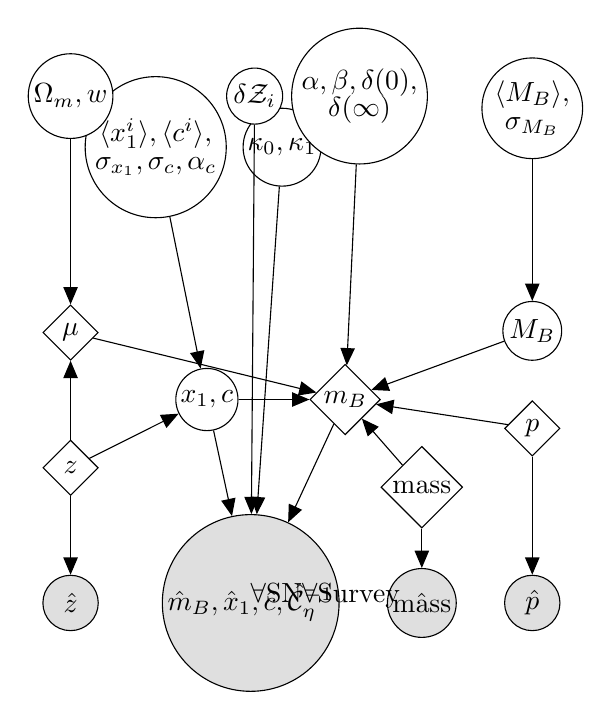
\begin{tikzpicture}
	% Obs nodes
	\node[obs]  (obssum) {$\hat{m}_B, \hat{x}_1, \hat{c}, \hat{\mathcal{C}}_\eta^{-1}$};
	\node[obs, left=0.8cm of obssum]  (zobs) {$\hat{z}$};
	\node[obs, right=0.6cm of obssum]  (mobs) {$\hat{{\rm mass}}$};
	\node[obs, right=0.6cm of mobs]  (pobs) {$\hat{p}$};
	% Latent nodes
	\node[det, above=of obssum, xshift=1.2cm] (mb) {$m_B$};
	\node[latent, left=of mb, xshift=0.1cm] (x1c) {$x_1, c$};
	\node[det, above=of zobs] (z) {$z$};
	\node[det, above=of mobs, yshift=-0.5cm] (m) {${\rm mass}$};
	\node[det, above=of pobs, yshift=0.5cm] (p) {$p$};	
	\node[det, above=of z] (mu) {$\mu$};
	\node[latent, above=of p, yshift=-0.5cm] (MB) {$M_B$};
	% Survey nodes
	\node[latent, above=of x1c, yshift=0.9cm, xshift=-0.65cm, align=center] (pop1) {$\langle x_1^i \rangle, \langle c^i \rangle, $\\$ \sigma_{x_1}, \sigma_c, \alpha_c$ };

	\node[latent, right=0.2cm of pop1, align=center] (kappa) {$\kappa_0, \kappa_1$};
	% Global nodes
	\node[latent, above=2.1cm of mu]  (cosmo) {$\Omega_m, w$};
	\node[latent, above=1.8cm of MB, xshift=0cm, align=center]  (MBpop) {$\langle M_B \rangle,$ \\ $\sigma_{M_B}$};
	\node[latent, right=1.43cm of cosmo, align=center]  (dz) {$\delta \mathcal{Z}_i$};
	\node[latent, right=0.1cm of dz, align=center] (ab) {$\alpha, \beta, \delta(0)$, \\$\delta(\infty)$};
	% Connect the nodes
	\edge {mb, x1c, dz, kappa} {obssum};
	\edge {z} {zobs};
	\edge {m} {mobs};
	\edge {p} {pobs};
	\edge {z,cosmo} {mu};
	\edge {MBpop} {MB};	
	\edge {MB, mu, ab, m, p, x1c} {mb}
	\edge {pop1, z} {x1c};

	% Plates
	\plated[thick] {sn} {(mb)(obssum)(zobs)(mobs)(pobs)(x1c)(z)(mu)(MB)(m)(p)} {$\forall\ \rm{SN}$} ;
	\plated[thick] {survey} {(sn)(pop1)(kappa)} {\\$\forall\ \rm{Survey}$} ;
	\end{tikzpicture}
\end{document}